\documentclass[aspectratio=43,9pt]{beamer}
%
\let\Tiny=\tiny
%
\usepackage{tikz}
\usepackage{enumerate}
%
\usetheme{Boadilla}
%
%
\let\Tiny=\tiny%			% to avoid warnings about font size
%\usepackage{lmodern}%		% alternative method to avoid these warnings
%
\catcode`~=11 % make LaTeX treat tilde (~) like a normal character
\newcommand{\urltilde}{\hbox{~}}
\catcode`~=13 % revert back to treating tilde (~) as an active character
%
% misc commands
\newcommand{\bm}[1]{\mathbf{#1}}
\newcommand{\bs}[1]{\boldsymbol{#1}}
\newenvironment{myitemize}[1]{\vspace{#1}\begin{itemize}\setlength\itemsep{#1}}{\end{itemize}}
%
% pgf markers
\usepgflibrary{plotmarks}
%
\setbeamertemplate{footline}
{
  \leavevmode%
  \hbox{%
  \begin{beamercolorbox}[wd=.8\paperwidth,ht=2.25ex,dp=1ex,left]{author in head/foot}%
    \usebeamerfont{author in head/foot}\hspace*{4em}\inserttitle
  \end{beamercolorbox}%
  \begin{beamercolorbox}[wd=.2\paperwidth,ht=2.25ex,dp=1ex,right]{author in head/foot}%
    \usebeamerfont{author in head/foot}\insertframenumber{} / \inserttotalframenumber\hspace*{1ex}
  \end{beamercolorbox}}%
  \vskip0pt%
}
%
\setbeamertemplate{navigation symbols}{}
%
\setbeamertemplate{frametitle}
{%
	\begin{minipage}{.9\paperwidth}
		\vspace*{1ex}%
		\flushright%
		%\bfseries
		\LARGE%
		\insertframetitle%
	\end{minipage}%
}
%
\setbeamertemplate{title page}{
	\begin{center}
		\vspace*{2ex}
		\usebeamercolor[fg]{frametitle}{%
			\Large%
			Numerical Techniques 2025--2026\\[2ex]
			%
			\LARGE%
			\inserttitle
		}\\[6ex]
		\usebeamercolor[fg]{normal text}{%
			Daan Degrauwe\\[1ex]
			\texttt{daan.degrauwe@meteo.be}\\[4ex]
			Postgraduate Studies in Weather and Climate Modeling\\[1ex]
			Ghent University
		}
	\end{center}
}
%
\newcommand{\ft}[2]{{\textstyle\frac{#1}{#2}}}
%
% increase space around equations
\makeatletter
\g@addto@macro\normalsize{%
	\setlength{\abovedisplayskip}{3ex}%
	\setlength{\belowdisplayskip}{3ex}%
	\setlength{\abovedisplayshortskip}{3ex}%
	\setlength{\belowdisplayshortskip}{3ex}%
}%
\makeatother
%

%
\graphicspath{{./figures/assignments}}
%
\title{Student projects}%
%
%%%%%%%%%%%%%%%%%%%%%%%%%%%%%%%%%%%%%%%%%%%%%%%%%%%%%%%%%%%%%%%%%%%%%%
%
\begin{document}
%
%%%%%%%%%%%%%%%%%%%%%%%%%%%%%%%%%%%%%%%%%%%%%%%%%%%%%%%%%%%%%%%%%%%%%%%%%%%%%%%%%%%%%%%%%%%%%%%%%%%%
%
\begin{frame}[plain]
	\titlepage
\end{frame}
%
%\begin{frame}
%
%[CHEBYSHEV: EXPLAIN THAT NOT THAT DIFFERENT FROM FOURIER: T\_n(cos(theta)) = cos(n.theta) ]
%[CHEBYSHEV: REF. TO NUMERICAL RECIPES]
%[Explain Davies perfect model experiments better, perhaps in separate document]
%[Provide Pierre's work on background state as reference for SI-SWE]
%
%\end{frame}
%
%%%%%%%%%%%%%%%%%%%%%%%%%%%%%%%%%%%%%%%%%%%%%%%%%%%%%%%%%%%%%%%%%%%%%%
%
\begin{frame}
	%
	\frametitle{General idea}
	%
	\begin{center}
		\bf Starting from a simple model, apply some\\
		of the techniques from this course.
	\end{center}
	%
	\par\vspace*{4ex}
	General remarks:
	%
	\begin{myitemize}{1ex}
		\item no course on Fortran or Linux; no course on complex algebra;\\ask for help!
		\item it's allowed to use Matlab, Python, R, etc. if you prefer this instead of Fortran;
		\item open assignment: no exact solution $+$ discussion is more important than results
		\item the purpose is you \emph{learn} something
		\item try to trigger strange/unwanted phenomena, and discuss solutions.
		\item you can propose a topic yourself.
	\end{myitemize}
	%
\end{frame}
%
%%%%%%%%%%%%%%%%%%%%%%%%%%%%%%%%%%%%%%%%%%%%%%%%%%%%%%%%%%%%%%%%%%%%%%
%
\begin{frame}
	%
	\frametitle{Shallow Water Equations}
	%
	\begin{center}
		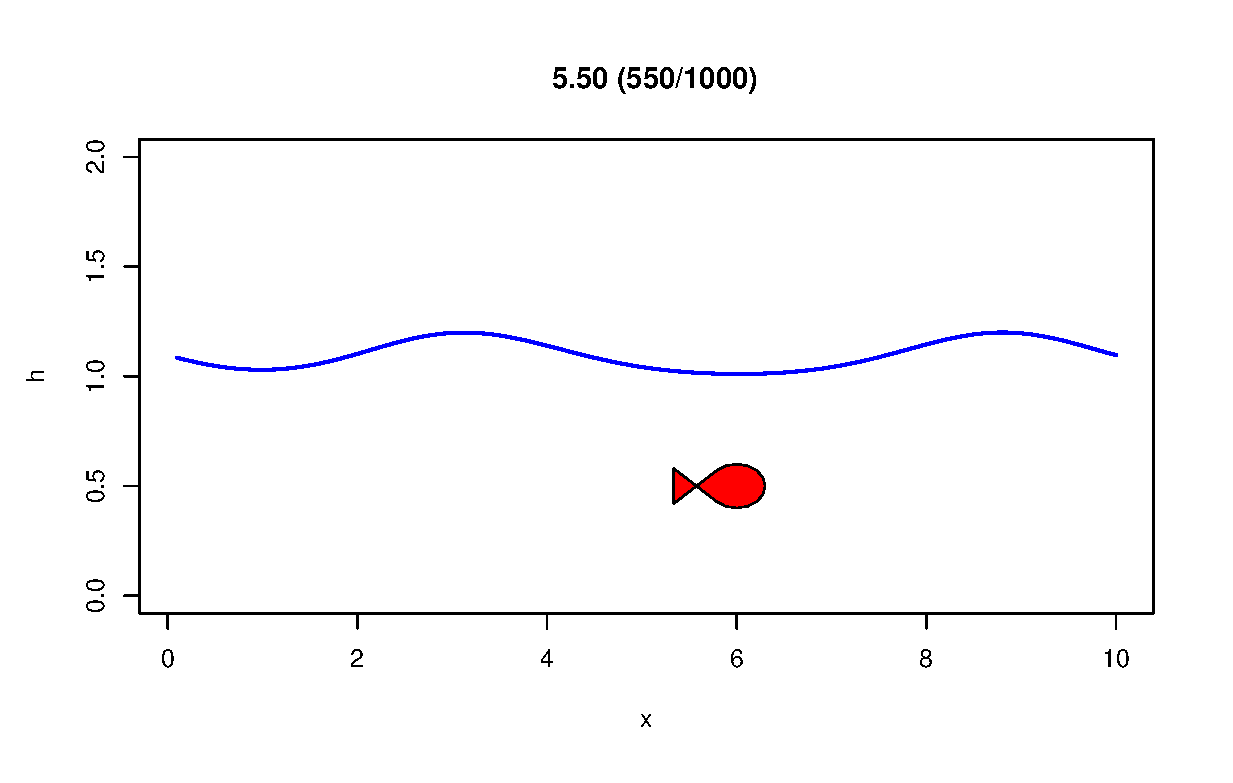
\includegraphics[width=9cm]{swe1D}
	\end{center}
	%
\end{frame}
%
%%%%%%%%%%%%%%%%%%%%%%%%%%%%%%%%%%%%%%%%%%%%%%%%%%%%%%%%%%%%%%%%%%%%%%
%
\begin{frame}
	%
	\frametitle{Shallow Water Equations}
	%
	The linearized 1D shallow water equations (SWE) are given by:
	%
	\begin{align*}
		\frac{\partial u}{\partial t}+U\frac{\partial u}{\partial x}+g\frac{\partial h}{\partial x}&=0\\
		\frac{\partial h}{\partial t}+H\frac{\partial u}{\partial x}+U\frac{\partial h}{\partial x}&=0
	\end{align*}
	%
	where $g$ is gravity, $U$ and $H$ are the constant basic-state velocity and water height, and $u(x,t)$ and $h(x,t)$ are the perturbations on the velocity and the water height.
	%
\end{frame}
%
%%%%%%%%%%%%%%%%%%%%%%%%%%%%%%%%%%%%%%%%%%%%%%%%%%%%%%%%%%%%%%%%%%%%%%
%
\begin{frame}
	%
	\frametitle{Shallow Water Equations}
	%
	The current model is very simple:
	%
	\begin{myitemize}{1ex}
		\item Leapfrog time integration
		\item Second-order centered space differencing
		\item Periodic boundary conditions
	\end{myitemize}
	%
	{\vspace*{4ex}\bfseries Student projects}:
	%
	\begin{myitemize}{1ex}
		\item[1.] Stagger $u$ and $h$
		\item[2.] Compare with nonlinear model
		\item[3.] Transform into spectral model with Fourier decomposition
		\item[4.] Transform into spectral model with Chebyshev decomposition\\[1mm]
			\quad J.P. Boyd, \emph{Chebyshev and Fourier Spectral Methods}\\
		\item[5.] Study Laplace transform integration\\[1mm]
			\quad\parbox{.9\textwidth}{Clancy and Lynch, 2011, QJRMS 137,\\\emph{Laplace transform integration of the shallow-water equations}}
	\end{myitemize}
	%
\end{frame}
%
%%%%%%%%%%%%%%%%%%%%%%%%%%%%%%%%%%%%%%%%%%%%%%%%%%%%%%%%%%%%%%%%%%%%%%
%
\begin{frame}
	%
	\frametitle{Barotropic Vorticity Equation}
	%
	\begin{center}
		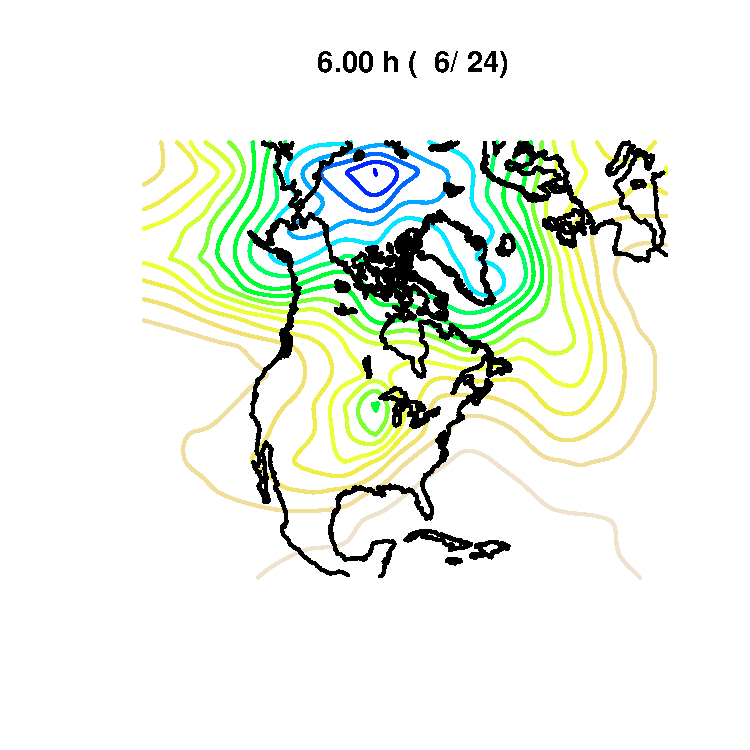
\includegraphics[width=7cm]{barovort}
	\end{center}
	%
\end{frame}
%
%%%%%%%%%%%%%%%%%%%%%%%%%%%%%%%%%%%%%%%%%%%%%%%%%%%%%%%%%%%%%%%%%%%%%%
%
\begin{frame}
	%
	\frametitle{Barotropic Vorticity Equation}
	%
	\begin{myitemize}{2ex}
		\item The barotropic vorticity equation BVE is given by:
			%
			\begin{equation*}
				\frac{\partial \zeta}{\partial t}+\bm u\cdot\nabla\zeta=0
			\end{equation*}
			%
			where $\zeta$ is the vorticity, and $\bm u$ is the geostrophic wind, given by
			%
			\begin{align*}
				\bm u&=\bm k\times\nabla\psi		&		\nabla^2\psi&=\zeta
			\end{align*}
			%
		\item Writing everything in terms of the streamfunction $\psi$, the BVE becomes
			%
			\begin{equation*}
				\frac{\partial\nabla^2\psi}{\partial t}+J(\psi,\nabla^2\psi)=0
			\end{equation*}
			%
			where $J$ is the Jacobian operator:
			%
			\begin{equation*}
				J(p,q)=\frac{\partial p}{\partial x}\frac{\partial q}{\partial y}-\frac{\partial p}{\partial y}\frac{\partial q}{\partial x}
			\end{equation*}
			%
	\end{myitemize}
	%
\end{frame}
%
%%%%%%%%%%%%%%%%%%%%%%%%%%%%%%%%%%%%%%%%%%%%%%%%%%%%%%%%%%%%%%%%%%%%%%
%
\begin{frame}
	%
	\frametitle{Some background info}
	%
	\begin{myitemize}{2ex}
		\item This model was used for the first numerical weather prediction in 1950 on the ENIAC computer
			%
			\begin{center}
				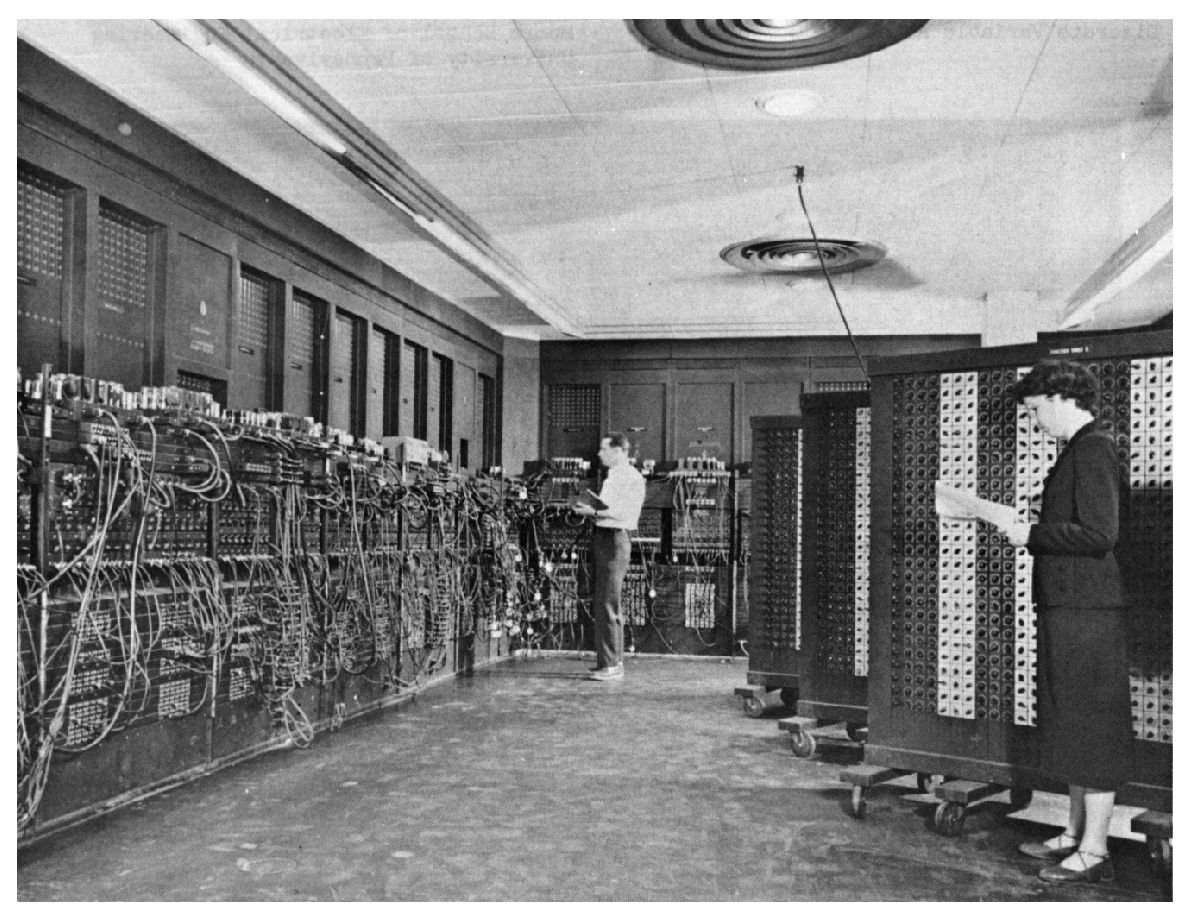
\includegraphics[width=5cm]{ENIAC}
			\end{center}
			%
		\item A 24-hour forecast took about 24h computing time
			%
	\end{myitemize}
	%
\end{frame}
%
%%%%%%%%%%%%%%%%%%%%%%%%%%%%%%%%%%%%%%%%%%%%%%%%%%%%%%%%%%%%%%%%%%%%%%
%
\begin{frame}
	%
	\frametitle{Original model}
	%
	The original (1950) model is characterized by:
	%
	\begin{myitemize}{1ex}
		\item a leapfrog time integration
			%
		\item second-order centered space differences
			%
		\item an expensive (pseudo-spectral) way to invert the Laplacian operator
			%
		\item heuristic boundary conditions:
			%
			\begin{myitemize}{1ex}
				\item $\frac{\partial \psi}{\partial t}=0$ on boundary
				\item $\frac{\partial \nabla^2 \psi}{\partial t}=0$ for entering fluid
			\end{myitemize}
			%
	\end{myitemize}
	Due to these boundary conditions and aliasing, the model is not stable.
	%
	\par\vspace*{4ex}
	The student's model is somewhat simplified:
	%
	\begin{myitemize}{1ex}
		\item Spectral inversion of Laplacian
		\item Periodic boundary conditions
		\item Coriolis effect removed
		\item Projection impact removed
	\end{myitemize}
	%
\end{frame}
%
%%%%%%%%%%%%%%%%%%%%%%%%%%%%%%%%%%%%%%%%%%%%%%%%%%%%%%%%%%%%%%%%%%%%%%
%
\begin{frame}
	%
	\frametitle{Improvements (student projects)}
	%
	General remark: lots of interesting aspects in this model, but you'll have to dig deeper to find them.
	%
	\par\vspace*{4ex}
	{\bf Student projects:}
	\begin{myitemize}{1ex}
		\item[6.] Semi-Lagrangian scheme
		\item[7.] High-resolution LAM nested in low-resolution LAM (coupling with Davies relaxation)
		\item[8.] Spectral model and avoiding aliasing
		\item[9.] Check energy cascade between large and small scales, and implement Arakawa Jacobian
	\end{myitemize}
	%
\end{frame}
%
%%%%%%%%%%%%%%%%%%%%%%%%%%%%%%%%%%%%%%%%%%%%%%%%%%%%%%%%%%%%%%%%%%%%%%
%
\begin{frame}
	%
	\frametitle{Practical aspects}
	%
	\begin{myitemize}{2ex}
		\item Groups of 2/3 persons
			%
		\item Pick a single topic (e.g. SWE-spectral)
			%
		\item More detailed background info (papers) on Ufora.
			%
		\item Support sessions: 18 April, 14h30; come prepared!
			%
		\item Report (say 5--10 pp.): deadline Sunday 24 April.
		\item Presentation for other students: Tuesday 25 April.
	\end{myitemize}
	%
\end{frame}
%
%%%%%%%%%%%%%%%%%%%%%%%%%%%%%%%%%%%%%%%%%%%%%%%%%%%%%%%%%%%%%%%%%%%%%%
%
\begin{frame}
	
	\frametitle{Getting started}
	
	\begin{myitemize}{3ex}
		\item Instead of working under Linux (previous years), we'll use a Jupyter notebook. Hopefully this is more student-friendly.
			%
		\item However, the actual model is still written in Fortran, but compiling, launching and reviewing results will be done from the Jupyter notebook.
			%
		\item To get started, take the following steps:\vspace*{2ex}
			%
			\begin{enumerate}
				\item login on the UGENT HPC infrastructure \texttt{https://login.hpc.ugent.be/}\vspace*{2ex}
				\item launch a Jupyter IPython Notebook (under Interactive Apps)\vspace*{2ex}
				\item \textbf{Make sure to use the following settings}:
					\begin{itemize}
						\item Set Cluster to `slaking'
						\item Choose an appropriate value for the Time (you will be kicked off the system after this time)
						\item Set IPython version to `7.15.0 foss 2020a Python 3.8.2'\vspace*{2ex}
					\end{itemize}
				\item Hit the `Launch' button at the bottom\vspace*{2ex}
				\item After a few minutes, you should be able to connect to your Jupyter job (under My Interactive Sessions)
			\end{enumerate}
	\end{myitemize}
	
\end{frame}
%
%%%%%%%%%%%%%%%%%%%%%%%%%%%%%%%%%%%%%%%%%%%%%%%%%%%%%%%%%%%%%%%%%%%%%%
%
\begin{frame}
	%
	\frametitle{Getting started with the Jupyter notebook}
	%
	\begin{itemize}
		\item The previous steps should bring you to an interface like this\vspace*{2ex}
			%
			\begin{center}
				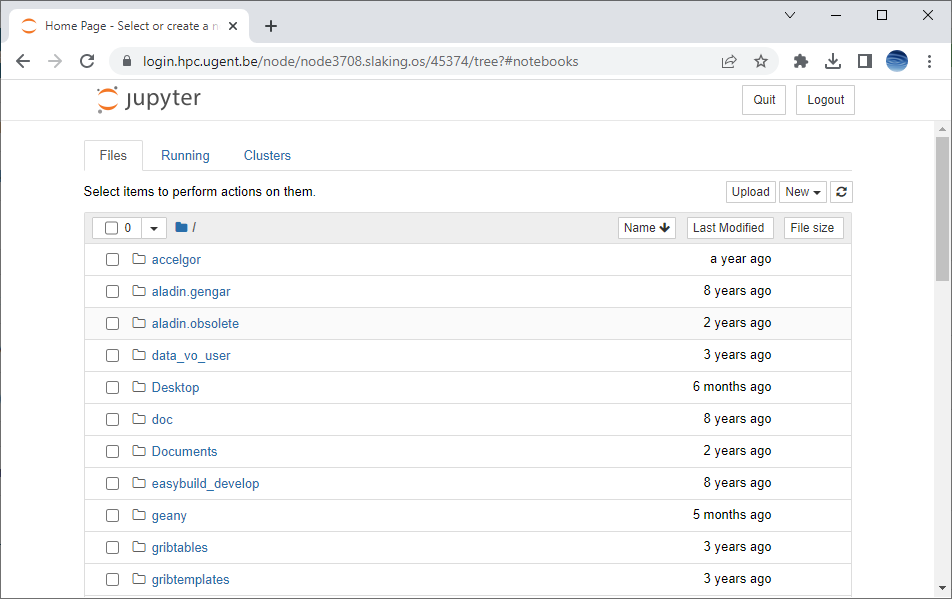
\includegraphics[width=.6\textwidth]{jupyter_home}
			\end{center}\vspace*{3ex}
			%
		\item This is not yet the actual notebook, but it allows you to easily navigate between files/folders, and to create new notebooks, folders or files.
	\end{itemize}
	%	
\end{frame}
%
%%%%%%%%%%%%%%%%%%%%%%%%%%%%%%%%%%%%%%%%%%%%%%%%%%%%%%%%%%%%%%%%%%%%%%
%
\begin{frame}
	%
	\frametitle{Getting started with the Jupyter notebook}
	%
	\begin{itemize}
		\item Since file/folder manipulation is easier in a Linux terminal window, launch a terminal (under New $\rightarrow$ Terminal).\vspace*{3ex}
		\item Create a new folder and copy the necessary files with\\[2ex]
			\begin{minipage}{\textwidth}
				\texttt{mkdir project\_numtech}\\
				\texttt{cp -r /user/gent/407/vsc40744/ugent/projects/swe1D project\_numtech/}
			\end{minipage}\\[2ex]
			(replace \texttt{swe1D} with \texttt{barovort} if needed)\\
			You can close the terminal window now.\vspace*{3ex}
		\item Back in the Jupyter launch window, navigate to the folder you just created. When clicking a Fortran file, an editor will open so you can modify it.\vspace*{3ex}
		\item Finally, click on the file \texttt{swe1D.ipynb}. This will open the notebook where you can interactively launch experiments and review the results.
	\end{itemize}
	%	
\end{frame}
%
%%%%%%%%%%%%%%%%%%%%%%%%%%%%%%%%%%%%%%%%%%%%%%%%%%%%%%%%%%%%%%%%%%%%%%
%
\begin{frame}
	%
	\frametitle{Getting started with the Jupyter notebook}
	%
	\begin{myitemize}{2ex}
		\item A notebook is organized in `Cells' containing python code. The code in a cell is evaluated when hitting the Run button or pressing Ctrl-Enter.
			%
		\item The SWE notebook contains 4 cells:
			%
			\begin{itemize}
				\item A cell to load the necessary functions from the module in the python file \texttt{swe1D\_fun.py}\vspace*{1ex}
				\item A cell to launch the model and retrieve the results (more on this later)\vspace*{1ex}
				\item A cell to animate the water height in time\vspace*{1ex}
				\item A cell to plot the water height at the last timestep
			\end{itemize}
			%
		\item What actually happens in the second cell is the following:
			%
			\begin{enumerate}
				\item the function \texttt{run\_program} from is called from the \texttt{swe1D\_fun} module.\vspace*{1ex}
				\item this function in turn launches a Linux script \texttt{run.sh}\vspace*{1ex}
				\item this script in turn performs the compilation with \texttt{gfortran} and runs the program\vspace*{1ex}
				\item the program generates an output file \texttt{output.dat}\vspace*{1ex}
				\item the function \texttt{run\_program} reads the data from this output file and transforms it into numpy arrays, which can be easily plotted.\vspace*{1ex}
			\end{enumerate}
			%
			While this looks quite combersome, *in principle* it shouldn't be modified. Only the Fortran code itself and the postprocessing in Jupyter need modifications.\vspace*{1ex}
			%
			\par
			Should something look strange or unexpected (and it will!) don't hesitate to contact me!
	\end{myitemize}
	%	
\end{frame}
%
%%%%%%%%%%%%%%%%%%%%%%%%%%%%%%%%%%%%%%%%%%%%%%%%%%%%%%%%%%%%%%%%%%%%%%
%
\end{document}
